\pagenumbering{arabic}
\chapter{Einleitung}
\label{c:intro}

Inhalt dieser wissenschaftlichen Arbeit ist das automatische Erstellen einer Material-Kostengliederung aus einer \ac{ifc}-Datei mithilfe von \ac{nlp} zur Erweiterung einer Bausoftware. Diese Bausoftware ist die ORCA AVA aus dem mittelständigen Softwarehaus \glqq ORCA Software GmbH\grqq{} aus Neubeuern. 
In diesem Kapitel soll eine kurze Einführung über die \glqq ORCA Software GmbH\grqq{} und das Produkt  ORCA AVA gegeben werden. Außerdem wird die Motivation für die Programmerweiterung und die wissenschaftliche Vorgehensweise dieser Arbeit beschrieben.

\section{Ausgangssituation}
\label{c:intro:start}

Die im Titel beschriebene Bausoftware ist die ORCA AVA aus dem Softwarehaus \glqq ORCA Software GmbH\grqq{}. Dieses wurde im Jahr 1990 von Dipl.-Ing. Siegfried Tille und Dipl.-Ing. Heinz Nießen gegründet. Der Hauptsitz des Unternehmens ist in Neubeuern, bei Rosenheim. Das Unternehmen ist auf die Produktentwicklung von Software für die Baubranche spezialisiert. Im Vordergrund stehen die Ausschreibungssoftware ORCA AVA und die Ausschreibungstext-Plattform AUSSCHREIBEN.DE. Ziel der Entwicklung ist es die \ac{ava} eines Bauvorhabens für Planer, Architekten und Bauingenieure zu vereinfachen. Der Leitfaden ist, Software zu entwickeln, die jeder versteht, intuitiv bedienbar ist, einen optimalen Workflow gewährleistet und viele Import- und Exportmöglichkeiten für den Datenaustausch bietet.
Diese Arbeit fokussiert sich auf eine Erweiterung der ORCA AVA. Sie ist für alle Architektur- und
Ingenieurbüros, Wohnungsbaugesellschaften, Unternehmen und Behörden zur einfachen Abwicklung von Bauprojekten mit Ausschreibung, Vergabe und Abrechnung. Zusätzlich bildet sie das Kostenmanagement von solchen Projekten ab. Die Software ist außerdem \ac{bim} fähig und bietet \ac{din} zertifizierte Schnittstellen für den Datenaustausch an. Neben der ORCA AVA gibt es den \ac{ifc}-Manager als eigene Instanz, der \ac{ifc}-Modelle anzeigen kann. Die ORCA AVA kann dann Mengen aus dem Gebäudemodell übernehmen.
Es stehen drei verschiedene Editionen der Software zur Verfügung. Die ORCA AVA \ac{se}, die ORCA AVA \ac{pe} und die ORCA AVA \ac{ee}. Die aktuellste Version ist die 25.0.

Technisch wird die ORCA AVA in .NET entwickelt. Ein Großteil der Anwendung besteht noch aus \ac{vb} Code. Alle neuen Komponenten und Erweiterungen werden in C\# implementiert. Neue \ac{gui}-Komponenten werden dementsprechend mit \ac{wpf} entwickelt. \ac{wpf} ist ein .NET Framework für das Erstellen von Windows Applikationen mit grafischer Benutzeroberfläche von Microsoft. \citep{Microsoft_2022} Die ORCA AVA und der \ac{ifc} Manager (siehe Abschnitt \ref{c:basics:ifc:usage}) laufen in eigenen Prozessen und kommunizieren auf Prozessebene in der lokalen Umgebung. 

\section{Motivation}
\label{c:intro:motivation}

Ziel der \glqq ORCA Software GmbH\grqq{} ist es, \ac{bim} noch mehr in die ORCA AVA zu integrieren. \ac{bim} bedeutet, dass die Planung von Bauprojekten vollständig auf digitaler Basis durchgeführt wird.  Für jeden Projektbeteiligten besteht somit jederzeit Zugriff auf alle projektrelevanten Daten über Kosten, Mengen und Zeitabläufen. Somit können Baukosten einfacher ermittelt und der Bauprozess besser überwacht werden. In Abbildung \ref{fig:bim} ist zu sehen, dass \ac{bim} ein relevanter Begriff in der Baubranche ist. Die Verwendung der Praxis ist allerdings noch nicht verbreitet. \citep[p.~20]{Thomas_Baumanns_Dr_Philipp-Stephan_Freber_Dr_Kai-Stefan_Schober_Dr_Florian_Kirchner2016-gu} Mit dem \glqq \ac{ifc} First\grqq{} Ansatz ist das langfristige Ziel der ORCA AVA das Thema \ac{bim} noch mehr abzudecken. Aus den Daten eines 3D-Gebäudemodells soll automatisch ein Ausschreibungstext erstellt werden können. Bauteile aus dem Gebäudemodell sollen dann mit Kurztext, Langtext, Menge, Preis und vordefinierten Kostengliederungen in den Programmteil Bauelemente der ORCA AVA übernommen werden. Aufgrund der hohen Relevanz des Themas, spricht das Ganze viele Kunden an und stellt somit ein effektives Werbemittel für den Verkauf der Software dar. Ein Teil des langfristigen Ziels ist die Übernahme der Baumaterialien aus einer \ac{ifc}-Datei. Diese bietet die erste Kostengliederung für den \glqq \ac{ifc} First\grqq{} Ansatz. Die Übernahme von weiteren Daten aus dem \ac{ifc}-Modell können darauf aufgebaut werden.

\begin{figure}[h]
	\centering
	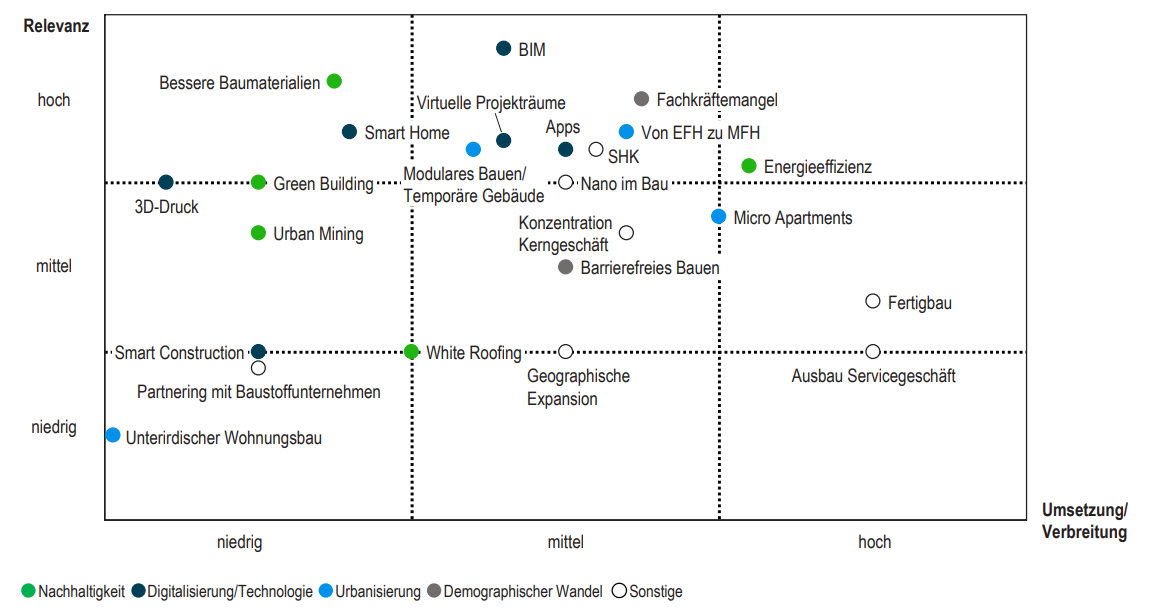
\includegraphics[scale=0.52]{bim-relevanz}
	\caption[Relevanz \ac{bim}]
	{Megatrends Nachhaltigkeit und Digitalisierung in der Bauwirtschaft. Bilder aus \citep[p.~20]{Thomas_Baumanns_Dr_Philipp-Stephan_Freber_Dr_Kai-Stefan_Schober_Dr_Florian_Kirchner2016-gu}}
	\label{fig:bim}
\end{figure}
Ein weiterer Trendbegriff, der mit der Programmerweiterung abgedeckt werden soll, ist \glqq Künstliche Intelligenz\grqq{} und \glqq Maschinelles Lernen\grqq{}. Das Suchinteresse der beiden Themen ist in Abbildung \ref{fig:ki-ml-trend} zu sehen. Die Werte geben das Google-Suchinteresse relativ zum höchsten Punkt im angegebenen Zeitraum an. Der Begriff \glqq Maschinelles Lernen\grqq{} hat seit Anfang 2015 ein steigendes Suchinteresse. Bei \glqq Künstliche Intelligenz\grqq{} ist das Suchinteresse von Anfang 2017 bis Ende 2021 konstant hoch. Der starke Anstieg ab November 2022 ist signifikant und korreliert mit der Veröffentlichung der Software ChatGPT. Man erkennt insgesamt, dass das Interesse über die letzten Jahre stetig ansteigt. Die Abdeckung dieser Begriffe ist seit geraumer Zeit ein Wunsch der Vertriebsseite für den noch besseren Verkauf der Software. Die Erweiterung wäre der erste Einsatz von maschinellem Lernen. Es ist also zusätzlich auch ein Pilotprojekt in der ORCA AVA Entwicklung, um sich mit Machine-Learning-Algorithmen vertraut zu machen und Erfahrungen in diesem Themengebiet zu bekommen.

Durch die genannten Punkte ist die Programmerweiterung dem Kano-Modell nach als Begeisterungsfeature zuzuordnen. Die Kundenzufriedenheit steigt also exponentiell mit dem Erfüllungsgrad der Anforderung. (siehe Abbildung \ref{fig:kano-model}) Mit der Zeit wandelt sich es dann erst in ein Leistungsfeature und irgendwann in ein Basisfeature. \citep[p.~3-4]{Hölzing_2008} Es besteht also die Motivation die Erweiterung möglichst exklusiv zur Verfügung zu stellen. Es eignet sich somit sehr für die ORCA AVA \ac{ee} Edition.

\begin{figure}[h]
	\centering
	
	\begin{subfigure}{0.99\textwidth}
		\centering
	\includegraphics[width=1\textwidth]{künstiliche-intilligenz-trend}
		\caption{Suchinteresse: Künstliche Intelligenz}
		\label{FIG:ki-trend}
	\end{subfigure}
	\hspace{1cm}
	\begin{subfigure}{0.99\textwidth}
		\centering
	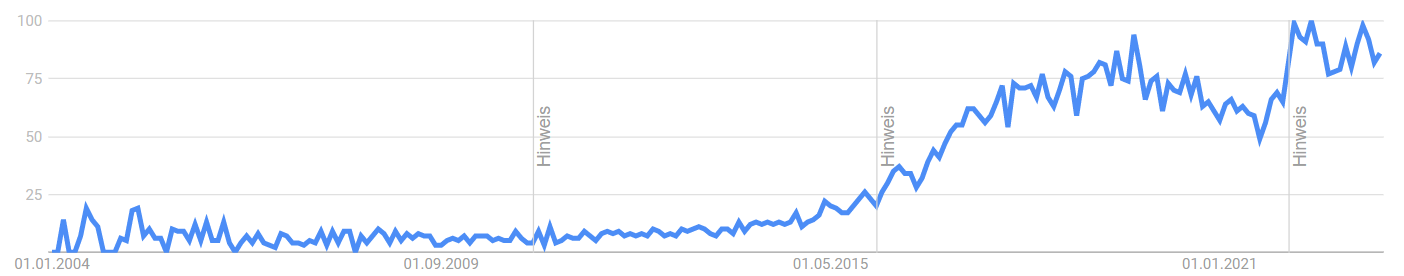
\includegraphics[width=1\textwidth]{machine-learning-trend}
		\caption{Suchinteresse: Machine Learning}
		\label{FIG:ml-trend}
	\end{subfigure}
	
	\caption[Google Trends]{Google Suchinteresse der beiden Begriffe \glqq Künstliche Intelligenz\grqq{} und \glqq Maschinelles Lernen{} seit 2004 bis 2023}
	\label{fig:ki-ml-trend}
\end{figure}

\begin{figure}[h]
	\centering
	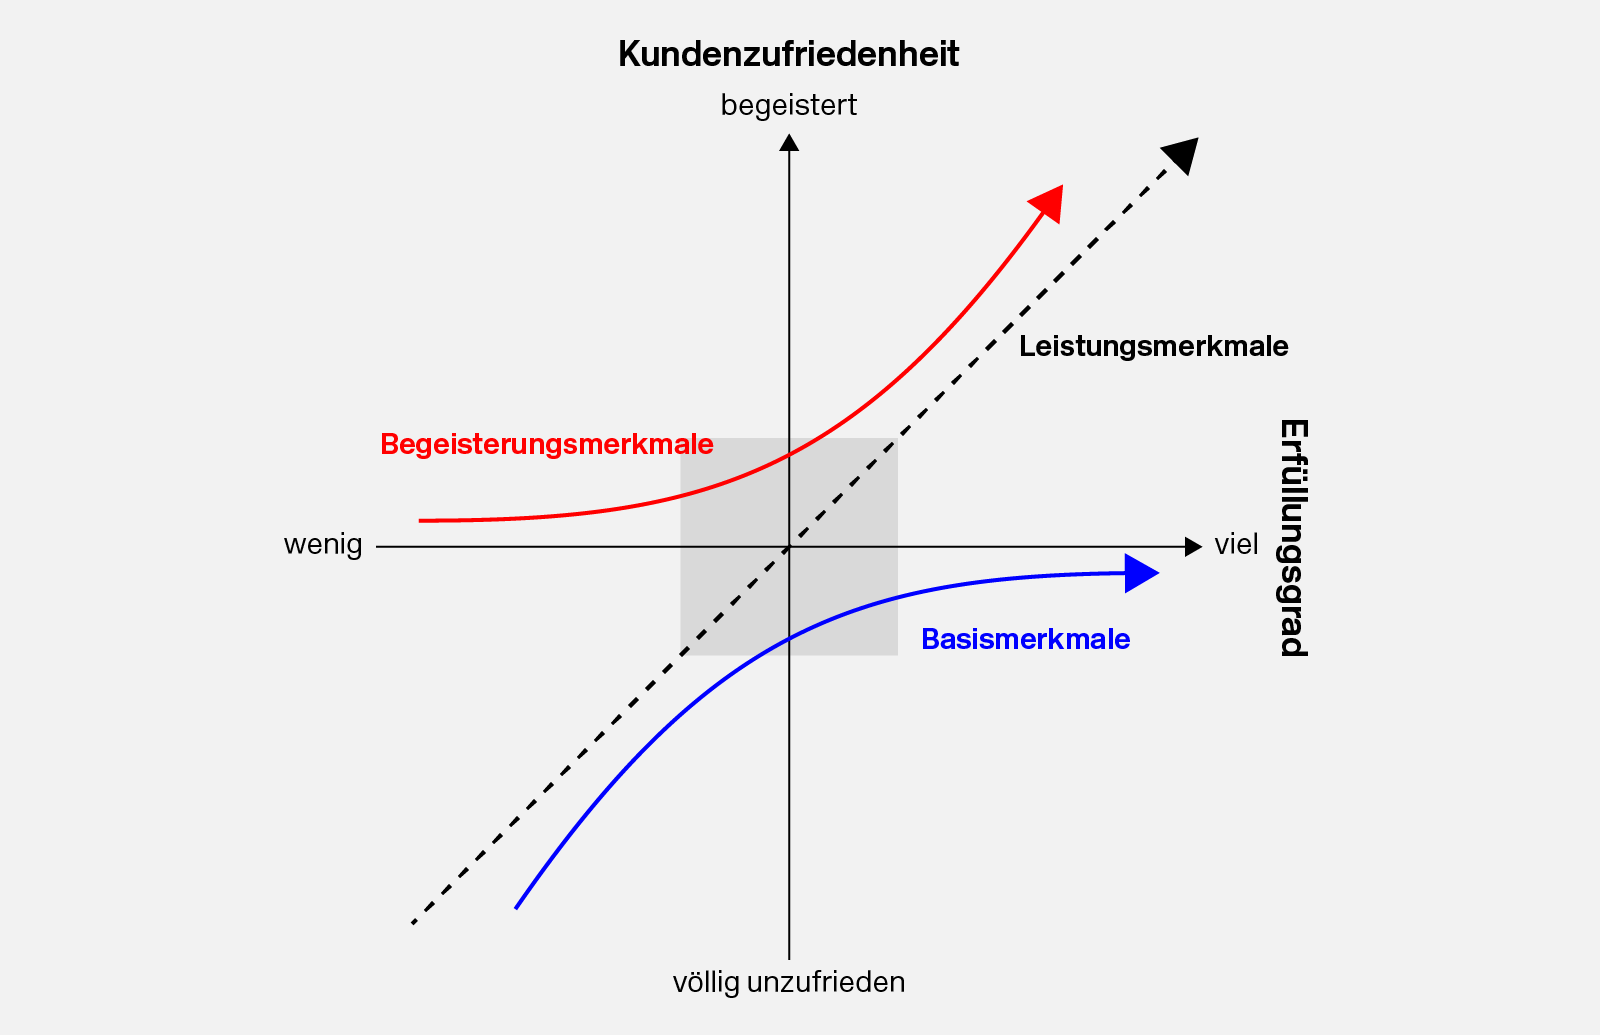
\includegraphics[width=\textwidth]{kano-modell}
	\quelle{https://dmexco-lightsails-media.s3.eu-central-1.amazonaws.com/wp-content/uploads/2021/01/04112832/Kano-Modell.png (Accessed: 2023-2-24) }
	\caption[Kano Modells]{Kano Modell der Kundenzufriedenheit}
	\label{fig:kano-model}
\end{figure}

\section{Ziel der Arbeit}
\label{c:intro:target}
Um die Anforderungen aus Abschnitt \ref{c:requirements:requirements} umsetzten zu können, muss zuvor ein Ziel formuliert werden.
Die Zieldefinition für diese Arbeit wird nach der SMART Technik definiert. Dabei muss ein Ziel folgende Eigenschaften haben:

\begin{itemize}
	%\setlength\itemsep{0.3em}
	\item Spezifisch
	\item Messbar
	\item Attraktiv
	\item Realisierbar
	\item Terminiert
\end{itemize}

Anhand dieser Kriterien wurde folgendes Ziel definiert:


\goalshaded{Bis zum 15.06.2023 wird eine \glqq Draftprojekt\grqq{} mit allen vollständigen funktionalen Anforderungen für die ORCA AVA implementiert. Für die Implementierung werden passende Algorithmen nach den Kriterien der Messbarkeit (siehe Abschnitt \ref{c:requirements:requirements:functional}) ausgewählt. Zusätzlich sollen die Maßnahmen zur Qualitätssicherung (Kapitel \ref{c:qs}) durchgeführt werden und die Qualitätssicherungs-Abteilung alle Funktionen freigegeben haben.}

\section{Wissenschaftliche Vorgehensweise}
\label{c:intro:methodology:scientific_proceture}
Im Folgenden wird die wissenschaftliche Vorgehensweise der Arbeit aufgezeigt.
In Abschnitt\,\ref{c:intro} wurde bereits die Ausgangssituation beschrieben, das Entwickeln der Programmerweiterung motiviert und des Ziel dieser Arbeit definiert. Im nächsten Kapitel, Kapitel\,\ref{c:basics}, werden Grundlagen erläutert, auf die diese Arbeit aufbaut. Im anschließenden Kapitel\,\ref{c:requirements} sollen die Problemstellung und Anforderungen analysiert werden. Danach (Kaptiel\,\ref{c:theoretical}) wird eine Lösung für die Problemstellung theoretisch konzipiert und verschiedene mögliche Algorithmen analysiert. In Kapitel\,\ref{c:comparison} werden die Algorithmen gegenübergestellt und nach den definierten Kriterien ausgewählt. Kapitel\,\ref{c:qs} zeigt die genutzten Maßnahmen der Qualitätssicherung auf. Am Ende wird das Ergebnis bewertet und ein Ausblick gegeben.
\todo{Muss noch vervollständigt werden}

\chapter{Grundlagen}
\label{c:basics}
In diesem Kapitel werden die Grundlagen im Bereich der fachspezifischen Themen, Technik und Projektmanagement vermittelt. Das soll Verständnis für die folgenden Kapitel schaffen. Zuerst geht es um das Projektmanagement. Anschließend geht es um das Format \ac{ifc}, dessen Geschichte und dessen Nutzungsmöglichkeiten für diese Arbeit. Außerdem wird die Struktur und der Nutzen einer Kostengliederung in der ORCA AVA veranschaulicht.

\section{Projektmanagement}
\label{c:basics:project-management}
Bevor auf technische und fachliche Aspekte von \ac{ifc} und Kostengliederungen eingegangen wird, folgt die Einführung in das Projektmanagements mit SCRUM und \ac{devops}.

\subsection{Vorgehensmodell}
\label{c:basics:project-management:procedure_model}
Das Projekt wurde mithilfe agiler Softwareentwicklung durchgeführt. Im ORCA AVA Entwicklungsteam wird das SCRUM Modell verwendet. Die Entwicklung der Produkterweiterung in dieser Arbeit läuft in diesem SCRUM-Prozess.

\begin{definition}[Scrum]
	\glqq Scrum is a lightweight framework that helps people, teams and organizations generate value through adaptive solutions for complex problems. \grqq{} \citep[p.~3]{scrum_2020}
\end{definition}

SCRUM verwendet einen iterativen, inkrementellen Ansatz. So kann Sprint für Sprint aus gewonnenen Erfahrungen der Entwicklungsablauf optimiert werden. \citep{scrum_2020} Product Owner in der ORCA AVA Entwicklung ist die \glqq ORCA Software GmbH\grqq{}, in Vertretung des Produktmanagement-Teams. Die Umsetzung der Sprint-Ziele wird von einer Person implementiert.

\subsection{DevOps}
\label{c:basics:project-management:devops}
Die Bezeichnung \ac{devops} vereint die beiden Praktiken \glqq Development\grqq{}(Entwicklung) und \glqq Operations\grqq{}(Vorgänge). Die traditionelle Trennung von Entwicklung und Softwarebetrieb führt oft zu
Interessenskonflikten. Entwickler wollen stetig die Software verbessern und der Betrieb will Änderungen vermeiden, um die Stabilität des Systems zu gewährleisten. Durch \ac{devops} entsteht ein Softwareentwicklungsprozess, den man durch Praktiken wie Continous Integration, Continous Delivery, Continous Deployment, automatisiertes Teste, Infrastructure-as-Code und automatische Veröffentlichungen beschleunigt. DevOps steht auch für eine Entwicklungskultur mit offener Zusammenarbeit, Kommunikation, Transparenz und Eingestehen von Fehlern, um Konflikte im Team zu vermeiden. \citep{devops_2021} Im Entwicklungsteam der ORCA AVA wird diese Praktik umgesetzt. Die technischen Hilfsmittel, die für den DevOps Prozess verwendet werden, sind in Abschnitt \ref{c:qs:technical_aids} beschrieben.

\section{\ac{ifc}}
\label{c:basics:ifc}
Die Daten für die Material-Kostengliederung werden aus einem digitalem Gebäudemodell entnommen. Der öffentliche internationale Standard (ISO 16739-1:2018) für Gebäudemodelle ist \ac{ifc}. \citep{BuildingSMART_IFC4_doc} Dieser wird auch in der bestehenden ORCA AVA benutzt, um den Ausschreibungsprozess zu unterstützen. \ac{ifc} Dateien können geöffnet, angeschaut und Informationen über das Modell in die Hauptsoftware übernommen werden. Im folgenden Kapitel wird die Geschichte, das Format von \ac{ifc} und die Verwendung in der ORCA AVA erläutert.

\subsection{Geschichte}
\label{c:basics:ifc:history}
\ac{ifc} ist die Hauptleistung der buildingSMART International, Ltd.  Die non-profit Organisation will mit der Spezifikation den BIM Prozess fördern und voranbringen. \citep{BuildingSMART_IFC}
Angefangen hat die Organisation als der Verein \textit{Industrieallianz für Interoperabilität IAI e. V.} mit Sitz in Berlin. 1994 startete die Entwicklung an dem offenen Datenmodellstandard \ac{ifc}. Dieser sollte die Anforderungen der Industrie an Interoperabilität gerecht werden und eine gemeinsame Basis zum Austausch von Informationen durch verschiedenen Anwendungen schaffen. Im Zusammenhang mit \ac{bim} sollten Daten lesbar, editierbar für verschiedene Systeme durch den Bauprozess und kompletten Lebenszyklus eines Gebäudes geteilt werden. \citep{Laakso2012-oi} Nach einigen Prototypen wurde 1999 \ac{ifc} 2.0 veröffentlicht. Diese wurde bis 2007 mit der Version 2.3.0.1 stetig verbessert. Die Version 2.3 wird auch in heutigen Projekten noch verwendet. 2013 wurde \ac{ifc}4 veröffentlicht, welche mit der Version 4.0.2.1 die aktuellste, offizielle \ac{ifc} Version ist. Das Format wird weiterhin stetig weiterentwickelt. Neue Versionen stehen schon vor einer Abstimmung der \ac{iso}. \citep{BuildingSMART_history_2022} Es gibt folgendermaßen aktuell zwei offizielle Versionen. Beide werden in der Praxis benutzt und sind, wie in Abschnitt \ref{c:basics:ifc:usage} beschrieben, mit der ORCA AVA kompatibel.


\subsection{Format}
\label{c:basics:ifc:format}
Das \ac{ifc} Format kodiert folgende Daten:
\begin{itemize}
	\item Identität, Semantik, Attribute und Relationen von Objekten
	\item Abstrakte Konzepte wie Performance oder Kosten
	\item Prozesse wie z.B.Installationen und Operationen
	\item Personen wie z.B. Eigentümer oder Lieferanten
\end{itemize}
Die Spezifikation kann also für das Bauen, Betreiben oder Nutzen eines Gebäudes genutzt werden. \ac{ifc} ist ein Implementierungs-Unabhängiges Datenmodell, welches in verschiedenen Umgebungen und elektronischen Formaten benutzt werden kann. Es kann beispielsweise in eine relationales Datenbankschema gegossen oder auch als Dateiformat implementiert werden. Das weitverbreiteste Format ist \ac{spf} \citep{Laakso2012-oi,BuildingSMART_IFC}. \ac{spf} ist das kompakteste Format für den dateibasierten Import und Export von \ac{ifc}-Dateien. Die Dateiendung des Formates ist \glqq \textit{.ifc}\grqq{}. Des Weiteren kann \ac{ifc} als \ac{xml} oder ZIP Datei verwendet werden. \citep{BuildingSMART_IFC}

\subsection{Verwendung}
\label{c:basics:ifc:usage}
\begin{displayquote}
	\glqq Today, \ac{ifc} is typically used to exchange information from one party to another for a specific business transaction.\grqq{} \citep{BuildingSMART_IFC}
\end{displayquote}
In der ORCA AVA wird \ac{ifc} für das Einlesen und Übernehmen von Maßen und Mengen in die Ausschreibung verwendet. Es vereinfacht den Prozess, die in der \ac{cad}-Software erstellten Daten einfach in die Leistungsverzeichnisse der ORCA AVA zu überführen.
Die ORCA AVA kann \ac{ifc}-Dateien einlesen. Im \ac{ifc} Manager wird das 3D-Modell dann angezeigt. In dem geöffneten Fenster gibt es einige fachliche Ansichten, die jegliche \ac{ifc}-Daten nochmal fachlich abstrahieren. In den Ansichten können zum Beispiel bestimmte Maße oder die Anzahl verschiedener Bauteile, die aus dem \ac{ifc}-Modell berechnet werden, in die ORCA AVA übernommen werden. Auch alle im \ac{ifc} definierten Eigenschaften eines Bauteils sind in der Eigenschaften-Ansicht sichtbar. Hier kann man auch die Materialbezeichnung des Bauteils finden, die im Modell hinterlegt ist. In Abbildung\,\ref{fig:ifc-manager} ist die Oberfläche des \ac{ifc} Managers zu sehen. Man sieht die Materialangabe rechts unten im Eigenschaftenfeld unter dem 3D-Modell.

Für das Arbeiten mit \ac{ifc}-Dateien wird die open-source Bibliothek xbim-toolkit verwendet. Die .NET Bibliothek kann \ac{ifc}-Dateien lesen, schreiben und anzeigen. Außerdem unterstützt es bei der Berechnung von komplexer Geometrie, um die Modelldaten für Analysen nutzbar zu machen. Die Entwicklung der Bibliothek startete 2007 und läuft seit 2009 in Zusammenarbeit mit der Norhumbria Untiversity. Mittlerweile bildet es die Standards \ac{ifc2x3} und \ac{ifc4} zu 100\% ab. Zudem bietet es an, auch \ac{ifc2x3} Modelle über das \ac{ifc4} Interface anzuprogrammieren. Somit können mit einer Codebasis beide Formate abgebildet und unterstützt werden. \citep{Xbim_ltd_history}


\subsection{Möglichkeiten für die  Materialangabe eines Bauteils}
\label{c:basics:ifc:buildingmaterial}
In einem \ac{ifc}-Modell können Materialien auf unterschiedliche Weise einem Bauteil zugewiesen werden. Die Spezifikation bietet die Klasse \textit{IfcMaterial}. Diese bildet fachlich ein Material ab. Es hat die Attribute Name, Description und Category.\citep{ifc_material} Eine Instanz von \textit{IfcMaterial} kann mit einem Element oder Elementtyp über die \textit{IfcRelAssociatesMaterial} verbunden werden. Diese Zuweisung kann über verschiedene Weisen stattfinden. In Abbildung \ref{fig:material-single} ist eine direkte Zuweisung über das \textit{IfcRefAssociatesMaterial} zu sehen. Hier hängt das \textit{IfcMaterial} direkt am Element. 
Bei einer Platte mit mehreren Schichten kann das \textit{IfcMaterial} auch wie in Abbildung \ref{fig:layer-set} zu sehen an einem \textit{IfcMaterialLayerSet} zugewiesen sein. Jede Schicht hat hier seine eigene Dicke und eigene Materialangabe. 
Ein Träger kann das \textit{IfcMaterial} über ein \textit{IfcMaterialProfileSet} abgebildet haben. (siehe Abbildung \ref{fig:profile-set})
Bei zum Beispiel einer Tür können verschiedene Materialien des Rahmens und der Verglasung über das \textit{IfcMaterialConstituentSet} abgebildet werden. (siehe Abbildung \ref{fig:constituent-set}) \citep{ifc_material_association}
Zusätzlich gibt es noch ältere Möglichkeiten Materialangaben an ein Element zu binden. In \ac{ifc2x3} gibt es die Klasse \textit{IfcMaterialList} \citep{Thomas2007_MaterialList}. Diese Möglichkeit ist deprecated, in der Praxis kommt das \ac{ifc2x3} Format noch regelmäßig vor. Die \textit{IfcMaterialList} muss also auch beachtet werden.

Neben verschiedenen Verbindungen zu \textit{IfcMaterial} hat jedes Element bei \ac{ifc} auch verschiedene Property Sets. Property Sets sind Container, die Eigentschaften je nach ihrem Namensattribut enthalten. Einige Property Sets sind in der Spezifikation des \ac{ifc} Standards enthalten. Es können auch zusätzlich benutzerdefinierte Property Sets erfasst werden. Diese können auch Informationen über das Material eines Elements enthalten. \citep{ifc_property_set} Das PropertySet \textit{Pset\_MaterialConcrete} weist darauf hin, dass es sich z.B um Beton handelt.

\begin{figure}[h]
	\centering
	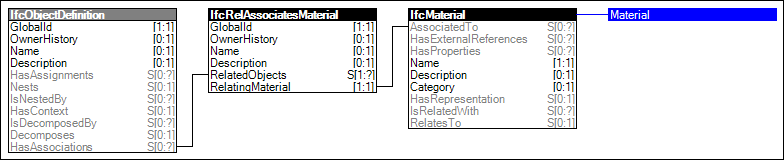
\includegraphics[width=\textwidth]{material-single}
	\caption[IfcMaterial]{Material Single Association}
	\label{fig:material-single}
\end{figure}

\section{Das Format Kostengliederung in der ORCA AVA}
\label{c:basics:coststructure}
Die Kostengliederung bietet eine Struktur, um Gesamtkosten einer Baumaßnahme in Kostengruppen unterteilt auswerten zu können. Logisch zusammengehörende Kosten können so in eine \ac{kg} zusammengerechnet werden. Außerdem handelt es sich beim Aufbau um eine Baumstruktur, wodurch Kostengruppen hierarchisch addiert werden können. In Abbildung \ref{fig:cost-structure} ist ein Beispiel einer Kostengliederung mit Materialien zu sehen. Der Gliederungspunkt \textit{Mineralisch} wird in die Unterpunkte \textit{Mauerwerk}, \textit{Beton}, \textit{Dachziegel} und \textit{Kies} unterteilt. Die Kosten der Unterpunkte können also für den Gliederungspunkt \textit{Mineralisch} addiert werden, um die Kosten aller Mineralien zu erfassen.
Bei einem Bauprojekt kann man so Kosten über alle Projektphasen vergleichen. Von der Kostenschätzung über die  Ausschreibung bis zur Rechnungsfreigabe. So können Kostenauswertungen nach den verschiedenen Kostengruppen durchgeführt werden. In einem ORCA AVA Projekt kann man verschiedene Kostengliederungen definieren. Es existieren bereits Standardkostengliederungen beim Erstellen eines neuen Projektes. Zusätzlich können neue Kostengliederungen erstellt oder importiert werden.\citep{helpdesk-kostengliederungen}


Technisch ist eine Kostengliederung als Modell im C\# Code definiert. Der Aufbau bildet die Baumstruktur über eine Referenz zur ParentNode und mehreren ChildrenNodes ab. Das Model kann über die ORCA AVA interne Middleware in der Datenbank persistiert werden. Die persistierten Kostengliederungen werden dann in entsprechenden Programmteilen angezeigt.
So müssen nach der generierten Kostengliederungs-Struktur die strukturierten Materialbezeichnungen in das C\# Modell abgebildet werden. So wird nach dem Import die erstellte Kostengliederung automatisch in der Oberfläche angezeigt und kann für Kostenauswertungen genutzt werden.


\chapter{Problemstellung und Anforderungen}
\label{c:requirements}
Im folgenden Kapitel werden die Problemstellung und Anforderungen aufgeführt, um das Projekt einzugrenzen. Diese kommen vom Auftraggeber, der \glqq ORCA Software GmbH\grqq{} selbst.

\section{Problemstellung}
\label{c:requirements:problem}

Die Problemstellung entsteht aus der Ausgangssituation (Abschnitt \ref{c:intro:start}) und der Motivation (Abschnitt \ref{c:intro:motivation}) der Bausoftware ORCA AVA. Der \ac{bim} Prozess soll noch mehr in die Software integriert werden. Deswegen wurde sich die Programmerweiterung der Materialkostengliederung gewünscht, um den ersten Schritt zu \glqq \ac{bim} First\grqq{} (siehe Abschnitt \ref{c:intro:motivation}) zu schaffen. Die Problemstellung dieser Arbeit bezieht sich der dementsprechenden Umsetzung dieser Programmerweiterung:

\begin{problem}
	\label{p:main}
	Wie lässt sich am besten eine Liste vom Materialbezeichnungen in eine hierarchische Material-Kostengliederung strukturieren?
\end{problem}

Da es sich hier um eine offene Frage handelt, sind Spielräume für die Antwort offen. Es soll ein Konzept und eine Architektur für die Programmerweiterung entstehen. Um ein fachlich richtiges Ergebnis der Strukturierung zu erreichen, ist aber vor allem folgende Problemstellung wichtig:

\begin{problem}
	\label{p:algorithm}
	Welcher \ac{nlp} Algorithmus eignet sich am besten für das Klassifizieren und Strukturieren von Material-Daten? 
\end{problem}

Bei dieser offenen Frage, soll am Ende ein Algorithmus aus einer Auswahl ausgewählt werden.
Um verschiedene Ansätze und Algorithmen vergleichen zu können, benötigt man Kriterien der Messbarkeit. Diese werden in Abschnitt \ref{c:requirements:requirements:functional} definiert. So kann man neben der Berücksichtigung der Anforderungen den geeignetsten Algorithmus für das Problem auswählen.

%\begin{problem}
%	\label{p:different-files}
%	Wie verhält sich die Variabilität der Materialangabe in verschiedenen %\ac{ifc}-Dateien für den jeweiligen Kostengliederungs-Import?
%\end{problem}

\section{Anforderungen}
\label{c:requirements:requirements}
Alle definierten Anforderungen kommen vom Projektmanagement Team der ORCA Software GmbH und dem Teamleiter der ORCA AVA Entwicklung. Die Gesamtheit von Anforderungen kann in funktionale Anforderungen, Leistungsanforderungen, spezifische Qualitätsanforderungen und Randbedingungen unterteilt werden.\citep{glinz_2007}

\subsection{Funktionale Anforderungen}
\label{c:requirements:requirements:functional}

\begin{definition}[Funktionale Anforderung]
	\label{d:functional-requirement}
	\glqq A functional requirement is a requirement	that pertains a functional concern.\grqq{}\citep{glinz_2007}
\end{definition}

Wie in Definition \ref{d:functional-requirement} beschrieben, geht es bei einer funktionalen Anforderung um die Funktion einer Software. Die im Mittelpunkt stehende Funktion ist die erläuterte Erstellung der hierarchischen Materialstruktur (Anforderung \ref{r:main}). Weitere Funktionen sind die Anforderungen \ref{r:takeover} und \ref{r:improvement}. Nach dem Importieren der Materialstruktur soll bei der Übernahme von Mengen die Materialkostengliederung automatisch zugewiesen werden. Zusätzlich sollen die Ergebnisse sich stetig verbessern. Dafür soll eine Möglichkeit geschafft werden, dass Nutzer der ORCA AVA Verbesserungen eintragen und somit den Datenbestand erweitern und verbessern.

\begin{requirement}
	\label{r:main}
	Aus einer Liste von Materialbezeichnungen soll eine hierarchische Baumstruktur entstehen, welche in einer ORCA AVA Kostengliederung benutzt werden kann.
\end{requirement}

\begin{requirement}
	\label{r:takeover}
	Bei der Übernahme einer Menge aus dem \ac{ifc} Manager soll die Materialkostengliederung zugewiesen werden.
\end{requirement}

\begin{requirement}
	\label{r:improvement}
	Bei schlecht generierter Struktur soll eine persistente, dauerhafte Verbesserung des Benutzers möglich sein.
\end{requirement}

Die in Anforderung \ref{r:main} generierte Materialkostengliederung soll fachlich möglichst richtig sein. Dazu werden folgende Kriterien der Messbarkeit definiert, um den genausten Algorithmus zu finden:

\paragraphheader{Genauigkeit}
Die Genauigkeit bei maschinellem Lernen misst die Wirksamkeit eines Modells. Klassifizierte Daten werden in einen Testdatensatz und einen Trainingsdatensatz geteilt. Mit dem Testdatensatz wird das trainierte Modell getestet und als Ergebnis der Genauigkeit hat man eine prozentuale Angabe der Übereinstimmung des Testdatensatzes. \citep{Microsoft_2022_ml}

\paragraphheader{Interpretierbarkeit}
\begin{definition}[Interpretierbarkeit]
	\label{d:interpretability}
	\glqq Interpretability is the degree to which a human can understand the cause of a decision.\grqq{}\citep{miller_2017}
\end{definition}
Hier geht es darum, die Ergebnisse des Algorithmus nachzuvollziehen zu können. Alleine die Genauigkeit reicht nicht dazu aus, einem Machine-Learning-Algorithmus vertrauen zu können.
Ein Modell ist besser interpretierbar als ein anderes Modell, wenn seine Entscheidungen für einen Menschen leichter nachvollziehbar sind als die Entscheidungen des anderen Modells. Die Interpretierbarkeit kann man nicht direkt messen. Sie entsteht aus der Erfahrung über den Algorithmus und die Nachvollziehbarkeit der vorhergesagten Ergebnisse durch Testen.  \citep{molnar2022} Das Endergebnis der Materialkostengliederungen aus verschiedenen Projekten, werden fachlich vom Produktmanagement bewertet. Diese habe das fachliche Wissen, um das Ergebnis bewerten zu können.

\paragraphheader{Robustheit}

Von Deep-Learning-Algorithmen erwartet man, dass sie robust gegen kleine Störungen in der Eingabe sind. Es wurde allerdings schon festgestellt, dass kleine Störungen teilweise das Ergebnis ändern können. \citep{Szegedy_2013} Im Bezug mit auf die Materialeingabe sollen zum Beispiel verschiedene Satzzeichen keinen Einfluss auf das Ergebnis haben. Die Materialbezeichnung \glqq Holz, Birke\grqq{} und \glqq Holz - Birke\grqq{} sollen mit dem Algorithmus auf das gleiche Ergebnis führen.

\paragraphheader{Performance}

Aspekte wie Geschwindigkeit und Ressourcenbedarf spielen eine sekundäre Rolle. Mit einem Fortschrittsbalken kann man dem Benutzer zeigen, dass es sich um einen zeitintensiven Algorithmus handelt. Wenn es den Anwendungsfluss allerdings sehr beeinträchtigt und verlangsamt, scheidet er als Option aus. Zum Punkt Performance zählt auch die Trainingsdauer des Algorithmus. Diese kann beim Verglich von verschiedenen Algorithmen helfen.\\

Die funktionalen Anforderungen werden noch nicht direkt in die ORCA AVA integriert. Ein Testprojekt soll zur Demonstration der Funktionen dienen. Es wird allerdings einen Vorschlag zur Integration in die Oberfläche der ORCA AVA geben. (siehe Kapitel \ref{c:closing:outlook})



\subsection{Weitere Anforderungen}
\label{c:requirements:requirements:additional}

Neben den funktionalen Anforderungen gibt es vor allem technische Anforderungen an die Programmerweiterung. Diese wurden vom Teamleiter der ORCA AVA Entwicklung gestellt:

\begin{requirement}
	\label{r:language}
	Die Programmerweiterung soll in .NET (C\#) oder in Python implementiert werden.
\end{requirement}

Die technische Einschränkung der Anforderung \ref{r:language} macht den Code und die Programmerweiterung für die ORCA Software GmbH wartbar. C\# ist die Hauptsprache der Firma. Zusätzlich gibt es auch schon Module in einem anderen Produkt mit Python. Für beide Programmiersprachen gibt es also schon Wissen in der Entwicklung, um bei Fehlerbehebungen eine erneute Einarbeitungszeit zu vermeiden.

\begin{requirement}
	\label{r:improvement}
	Die Strukturierung soll mit der Erweiterung der Datengrundlage immer besser gemacht werden können.
\end{requirement}

Durch das Einlesen neuer \ac{ifc}-Dateien von Benutzern, werden immer neue Materialbezeichnungen gesammelt, die die Datengrundlage erweitern. Dadurch müssen immer wieder neue Begriffe klassifiziert werden können, um das Modell stetig zu verbessern. Dementsprechend müssen \ac{ki}-Modelle auch immer wieder neu trainierbar sein. Diese Funktionen sollen also einem ORCA Internen Mitarbeiter zur Verfügung stehen.

Durch die beschriebenen Anforderungen aus Abschnitt \ref{c:requirements:requirements} entstand das beschriebene Ziel der Arbeit (siehe Abschnitt \ref{c:intro:target})

\chapter{Theoretische Konzeption}
\label{c:conception}
In diesem Kapitel wird ein theoretisches Konzept für das Lösen der Problemstellung erstellt und begründet. Zuerst wird das Konzept vorgestellt. Dann werden mögliche Algorithmen erläutert und evaluiert, wie sie zu den Anforderungen passen. Im Folgekapitel werden die Algorithmen miteinander verglichen und der geeignetste ausgewählt.

\section{Grundlegende Architektur und Vorgehensweise}
\label{c:conception:architecture}
In diesem Abschnitt wird das erarbeitete Konzept für die Erweiterung vorgestellt und begründet. In Abbildung \ref{fig:usecasediagramm} ist ein Anwendungsfalldiagramm der neuen Funktionen zu sehen. Die Anwendungsfälle des Benutzers der ORCA AVA decken sich mit den schon beschriebenen funktionalen Anforderungen (Abschnitt \ref{c:requirements:requirements:functional}) Die zusätzlichen Anwendungsfälle ergeben sich aus Anforderung \ref{r:improvement}.

\begin{figure}[h]
	\centering
	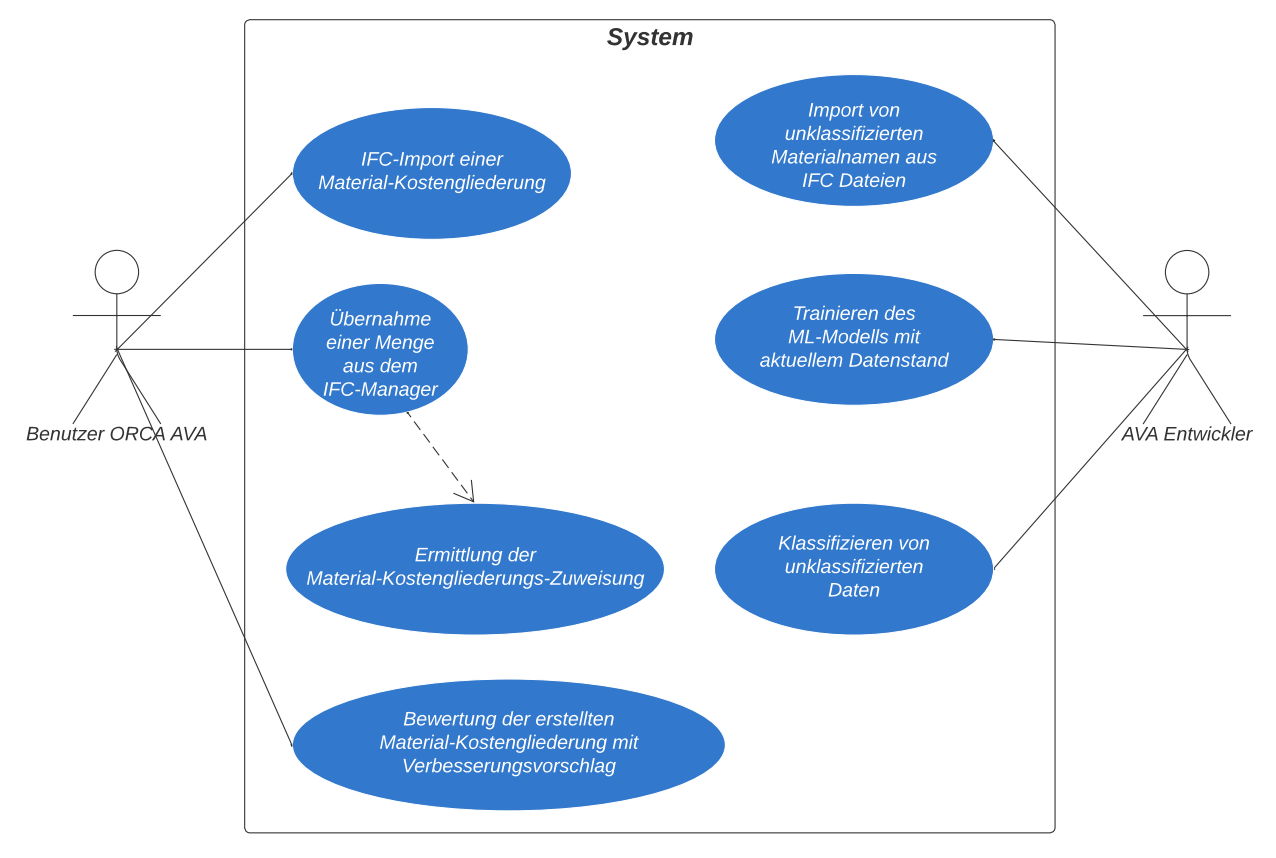
\includegraphics[width=\textwidth]{anwendungsfalldiagramm}
	\caption[Anwendungsfalldiagramm]{Anwendungsfalldiagramm}
	\label{fig:usecasediagramm}
\end{figure}

Das Ergebnis des Hauptanwendungsfalles der Material-Strukturierung ist abhängig von den Inhalten der \ac{ifc}-Datei. Durch die Nutzung verschiedener \ac{cad}-Programme und eigene Vorlieben bei der Materialangabe der ORCA AVA Benutzer entstehen viele unterschiedliche Inhalte bei der Materialangabe.
Um die hierarchische Strukturierung zu vereinfachen, werden Materialien zuerst nach dem \glqq Teile-und-hersche\grqq{} Verfahren in Oberkategorien klassifiziert. In Abbildung \ref{fig:material-categories} sind die Kategorien mit Beispielen aufgelistet. So müssen anschließend nur noch eine kleinere Liste von Materialien einer Oberkategorie weiter hierarchisch strukturiert werden.

In Abbildung \ref{fig:distribution-diagramm} ist ein Verteilungsdiagramm mit allen relevanten Objekten zu sehen. Auf dem Lokalem Computer des Benutzers laufen die beiden Prozesse der ORCA AVA und des \ac{ifc} Managers. Die ORCA AVA kommuniziert mit einem Webserver über \ac{rest}. Dieser verwaltet die anhängende SQL-Datenbank und übernimmt das Strukturieren des Material-Kostengliederungs-Import.

\subsection{Implementierung als Web-Service}
\label{c:conception:architecture:service}
Für die Materialstrukturierung ist ein neuer Webservice vorgesehen, mit den die ORCA AVA kommunizieren kann. Dies bietet einige Vorteile:

\begin{itemize}
	\setlength\itemsep{0.3em}
	\item Der Import greift immer auf das aktuellste \ac{ki}-Modell zu, welches zentral verwaltet werden kann
	\item Wegen der Verwendung von Python muss nicht bei jedem Client eine lauffähige Pythonumgebung vorhanden sein oder durchs Setup installiert werden.
	\item Neue Materialbezeichnungen und Klassifizierungen können direkt zentral Datenbank persistiert werden.
	\item Eine Änderung/Verbesserung der Datengrundlage kann durch automatisches Trainieren direkt zu einem verbessertem \ac{ki}-Modell führen.
\end{itemize}
Für die ORCA AVA bestehen schon Services für die Bereitstellung von News, die Lizenzierung oder das Updaten der Software. Durch die Vorgabe der ORCA Software GmbH wird der Service mit ASP.NET implementiert. ASP.NET ist ein Open-Source und Plattform-unabhängiges Web-Framework für die Entwicklung cloudbasierter Anwendungen wie Web-Applikationen, \ac{iot}-Apps oder mobile Backends. \citep{asp-net}. Die Architektur dieses Services entspricht dementsprechend den schon existierenden Services.

Daten werden über den Service in einem SQL-Datenbank Server gespeichert. Hier werden auch die ORCA Software GmbH internen Standards verwendet. Daten für den Material-Kostengliederungs-Import sind in der Tabelle \textit{Materials} persistiert. Die Tabellendokumentation ist in Abbildung \ref{fig:db-scheme} zu sehen. Zusätzlich bestehen Tabellen für die Autorisierung der Zugriffe auf den Service.

\begin{figure}[H]
	\centering
	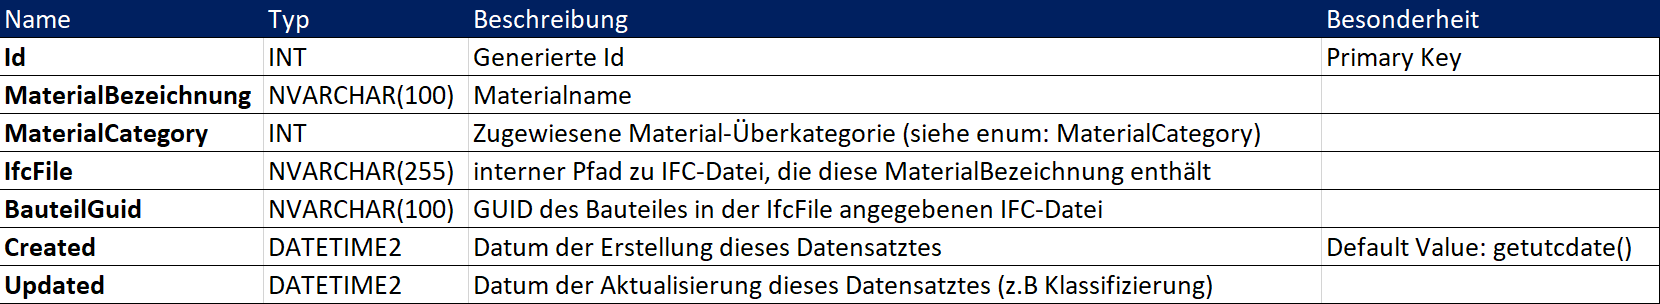
\includegraphics[width=\textwidth]{db-scheme}
	\caption[Dokumentation]{Dokumentation der Tabelle \textit{Materials} der Datenbank}
	\label{fig:db-scheme}
\end{figure}

\subsection{Konzept der Materialstrukturierung}
\label{c:conception:architecture:structuring}

\subsection{Konzept für das Auslesen von Materialien aus einer \ac{ifc} Datei}
\label{c:conception:architecture:ifc-material-extraction}
\section{Algorithmen für die Textklassifizierung}
\label{c:conception:classification}
\subsection{Ablauf einer Textklassifizierung}
\label{c:conception:classification:steps}

Das Klassifizieren von Texten teilt sich oft in die folgende Stufen. Alle diese Stufen wirken sich auf das Ergebnis der Klassifizierung aus:

\begin{figure}[H]
	\centering
	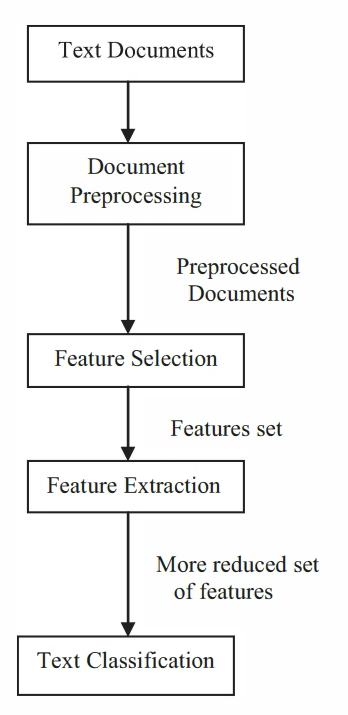
\includegraphics[width=0.3\textwidth]{classification-flow}
	\caption[Textklassifizierung]{Stufen der Textklassifizierung (Quelle:  \cite{Foram_2016})}
	\label{fig:classification flow}
\end{figure}

\paragraphheader{Preprocessing}
Das Preprocessing ist ein wichtiger Schritt vor der Klassifizierung. Es hat Auswirkungen auf die Genauigkeit, Interpretierbarkeit und Robustheit des Gesamtalgorithmus aus. \citep{Zelaya_2019} Materialbezeichnungen aus \ac{ifc}-Dateien können verrauscht und uneinheitlich sein, da es sich um ein Freitextfeld handelt. Die Vorverarbeitung der Daten hilft, die Daten zu säubern und auf das wesentliche reduzieren. \citep{Priyanga_2016}
Die Vorverarbeitungsstufe besteht normalerweise aus Aufgaben wie Tokenisierung, Entfernung von Stoppwörtern, Umwandlung in Kleinbuchstaben und Stemming. \citep{Uysal_2014}
Für die Materialklassifizierung werden zuerst bestimmte Zeichenketten rausgefiltert. Of befinden sich in der Bezeichnung Größen- und Farbangaben.
Mithilfe von Regex werden Farben, RGB-Farbcodes (z.B \textit{60 - 60 - 60}) und Größenangaben (z.B \textit{400 x 300}) aus dem String entfernt. Anschließend wird der Text in Tokens und jeder Token in Kleinbuchstaben umgewandelt. Aus \textit{\glqq Kunststoff - grau 80-80-80\grqq{}} wird dann z.B. \textit{\glqq 'kunststoff'\grqq{}} und aus \textit{\glqq Beton- C30/37 Verputzt\grqq{}} wird \textit{\glqq 'beton', 'c30/37', 'verputzt'\grqq{}}

\paragraphheader{Feature selection}
Da es bei der Materialstrukturierung nur ein Feature gibt, muss keine Auswahl aus einem Feature-Set getroffen werden. Es werden lediglich Größen- und Farbangaben aus dem Material-String im Preprocessing entfernt.

\paragraphheader{Feature extraction}
\begin{definition}[Feature extraction]
	\label{d:feature-extraction}
	\glqq Feature extraction addresses the problem of finding the most compact and informative set of features, to improve the efficiency or data storage and processing.\grqq{} \citep{Guyon2006}
\end{definition}
Zusätzlich werden in diesem Schritt beliebig formatierte Daten in eine  maschinenlesbare numerische Darstellung umgewandelt. \citep{scit-learn_featureextraction} Auch die im Preprocessing entstandenen Tokens sind noch Zeichenketten die in eine numerische Darstellung umgewandelt werden müssen.

\paragraphheader{Classification stages}
Nachdem die vorherigen Schritte auf die Daten ausgeführt wurde, kann die Klassifizierung starten.

\subsection{Sdca Maximum Entropy}
\label{c:conception:classification:sdca}
\subsection{Convolutional Neural Network}
\label{c:conception:classification:cnn}
\section{Möglichkeiten für die Feinstrukturierung}
\label{c:conception:fine-structuring}
\subsection{OpenAI Schnittstelle}
\label{c:conception:fine-structuring:openai}
OpenAI ist ein Unternehmen für \ac{ki}-Forschung und -Einsatz. Sie bieten verschiedene \ac{ki}-Modelle über eine \ac{api} an. Neben Speech-ToText und einem Bildgenerierungsmodell gibt es das Sprachverarbeitungsmodell \ac{gpt}
\subsection{FastText mit Density Based Clustering}
\label{c:conception:fine-structuring:dbscan}


\chapter{Gegenüberstellung der möglichen Konzepte}
\label{c:comparison}

\section{Vergleich der Textklassifizierung}
\label{c:comparison:classification}
\subsection{Messkriterien}
\label{c:comparison:classification:criteria}
\subsection{Auswahl eines Algorithmus}
\label{c:comparison:classification:selection}
\section{Vergleich der Feinstrukturierung}
\subsection{Messkriterien}
\label{c:comparison:fine-structuring:criteria}
\subsection{Auswahl eines Algorithmus}
\label{c:comparison:fine-structuring:selection}

\chapter{Praktische Umsetzung}
\label{c:implementation}
\section{Implementierung des Services}
\label{c:implementation:service}
\section{Python-Interop}
\label{c:implementation:python-interop}

\section{Implementieren des Auslesens aller Materialien aus einer \ac{ifc} Datei}
\label{c:implementation:ifc-material-extraction}

\section{Strukturieren der Materialnamen}
\label{c:implementation:structuring}
\subsection{Implementierung des Preprocessings}
\label{c:implementation:preprocess}
\subsection{Erstellen einer Datengrundlage}
\label{c:implementation:data}
\subsection{Training des Text-Klassifizierungsmodells}
\label{c:implementation:classification-training}
\subsection{Training des FastText Modells}
\label{c:implementation:embedding-training}
\subsection{DBSCAN Clustering}
\label{c:implementation:clustering}





\chapter{Maßnahmen zur Qualitätssicherung}
\label{c:qs}
\section{Clean Code}
\label{c:qs:cleancode}
\section{Technische Hilfsmittel}
\label{c:qs:technical_aids}
Bei der Durchsetzung von Maßnahmen der Qualitätssicherung wurden technische Hilfsmittel verwendet. Diese sind Visual Studio, Visual Studio Code, SonarQube, Azure DevOps und CI/CD. Auf diese wird in diesem Abschnitt eingegangen.
\section{Tests und Abnahme}
\label{c:qs:tests}


\chapter{Abschluss}
\label{c:closing}

\section{Bewertung der praktischen Umsetzung}
\label{c:closing:rating}
\section{Fazit}
\label{c:closing:conclusion}
\section{Integration in die ORCA AVA}
\label{c:closing:integration}
\section{Ausblick}
\label{c:closing:outlook}
Die Erweiterung soll in der Version 26 in der ORCA AVA Enterprise Edition erscheinen.
